\chapter{机器学习理论基础}
\label{chap:statistical-learning-framework}

用一批已标注的邮件训练垃圾邮件分类器，我们希望它也能判断以后收到的新邮件。但训练集上的准确率只检验了分类器对这些训练样本的预测：一个真正抓住了共同规律的分类器，和一个逐条背下训练样本的分类器，都可能在这里拿到高分。要判断学习是否成功，还必须看它们在没见过的邮件上犯多少错误。

把另一批邮件留作测试，可以估计当前这个分类器的错误率。但学习算法的保证还涉及另一层变化：如果重新抽取一批训练邮件，同一个算法可能选出不同的分类器，新分类器的表现也会随之波动。于是“有限的观测什么时候足以判断未来的错误率”这个问题，取决于三件事：训练样本和测试样本是怎么产生的、算法按什么规则选择结果、我们允许多大的预测误差和多高的训练失败概率。机器学习理论把这些关系写成明确条件，使“一次测试得到的结果”和“重复训练都成立的保证”能够分开分析。

本章要回答四个相互衔接的问题。第一，怎样把“学得好”说成可以证明或否证的陈述？为此先用邮件二分类把观测、假设和风险具体化，再用PAC标准给出成功的定义。第二，只追求训练错误最少为什么不够？记忆型反例和没有免费的午餐定理将说明，缺少对候选规则的限制，任何算法都无法统一成功。第三，限制候选规则要付出什么代价、限制多强才合适？风险分解与模型选择回答这一问题。第四，后续各章分别从哪个方向推进？本章最后按表达、收敛和泛化整理研究问题，并回顾其发展。第~\ref{chap:statistical-learning-framework}--\ref{chap:transfer-learning-theory}章都在这里建立的框架上展开。

\section{学习问题}
\label{sec:learning-problem}
\label{sec:statistical-learning-problem}

要讨论“未来的错误率”和“重复训练时的成功机会”，先得说清楚几样东西：算法看到的一条记录长什么样，一次判断怎样计分，算法从哪些规则里挑选，又拿什么作比较，数据和算法里的随机性各从哪里来。在邮件分类中，一条训练记录是一封邮件和它的标签，算法交付一个分类器，用未来的错误率评价它。回归和聚类中的对应对象不同，但需要回答的问题相同。本节先列出这些对象各自的职责，再用二分类逐一具体化，最后把风险和可学习性写成对一般任务都适用的形式。

\subsection{基本设定}
\label{sec:learning-problem-basic-setting}

先看算法收到的一条记录：邮件分类里是邮件及其类别，回归里是预测输入和真实数值，聚类里则是待分组的对象。所有允许出现的记录组成\emph{观测空间}（observation space），记为$Z$。指定$Z$时还要同时确定记录的单位：一封独立的邮件、一段前后相关的对话，还是一整块环境数据，所含的信息差别很大，不能不加分析地都当作“一条独立样本”来计数。

有了记录，还要回答“一次判断错得有多严重”。为此给每种“决策—观测”搭配指定一个数值代价，由\term{损失函数}（loss function）$\ell$计算：$\ell(w,z)$表示用决策$w$处理观测$z$时付出的代价，数值越小越好。分类中错分一次记多少、回归中偏差多大记多少，都由它规定。

接下来是“算法可以交出什么”和“拿什么作比较”。这两个问题初看是同一个，分开写是因为评价学习结果时总要问：它的风险和谁比算小？我们需要一组用作比较基准的候选决策，称为\emph{比较决策空间}（comparison decision space），记为$\mathcal W$；全部阈值分类器、只允许特定参数的回归函数、固定中心数的聚类方案，都可以组成这样一组基准。后文的“最低风险”和“超额风险”都相对$\mathcal W$计算。另一方面，算法实际被允许交出的决策组成\emph{输出决策空间}（output decision space），记为$\mathcal W_{\mathrm{out}}$。通常算法直接从基准候选中选一个，这时$\mathcal W_{\mathrm{out}}=\mathcal W$；但算法也可以交出候选之外的结果，例如把几个阈值组合成一条更复杂的规则，这时$\mathcal W_{\mathrm{out}}$比$\mathcal W$大。

据此可以区分两类学习。输出始终落在$\mathcal W$内，称为\term{恰当学习}（proper learning）；允许输出$\mathcal W$之外、但仍在$\mathcal W_{\mathrm{out}}$中的决策，称为\term{非恰当学习}（improper learning）。两者都以$\mathcal W$中的最低风险为基准，区别只在交出的决策是否必须属于$\mathcal W$。允许非恰当输出有时能让学习更容易，但比较基准不因此改变。

这里用“决策”这个总称，是因为框架还要覆盖回归、聚类等问题；在监督预测中，决策就是预测模型。因此，比较决策空间对应第~\ref{chap:machine-learning-models}章说的候选模型类$\mathcal H$，其中每个候选是一条完整的预测规则；学习规则最终选出的那条规则就是训练模型，而不是某一次预测返回的类别或数值。

最后要交代随机性。理论保证不是针对某一份具体数据，而是针对“可能遇到的数据来源”作出的，所以要先划定允许的来源范围，即\emph{允许的样本生成规律}；这个范围通常不告诉算法，算法只知道真实来源在其中。\emph{抽样机制}再规定训练观测彼此之间、以及训练观测与将来评价所用观测之间的关系，例如是否独立、是否来自同一来源。算法自身也可能使用随机数，例如并列时随机挑选或随机初始化，我们用一个独立于数据的随机量$U$记录它。把数据的随机性和算法的随机性分开写，才能分别讨论它们对最终保证的影响。下面把这些对象合进同一个形式设定。

\begin{definition}[学习问题的形式设定]
\label{def:learning-problem-setting}
一个学习问题至少需要规定观测空间$Z$、比较决策空间$\mathcal W$、输出决策空间
$\mathcal W_{\mathrm{out}}$、损失函数、允许的样本生成规律、抽样机制和算法可见的信息。

在$Z$与$\mathcal W^+=\mathcal W\cup\mathcal W_{\mathrm{out}}$上约定相应的可测结构，
并要求损失
\[
 \ell:\mathcal W^+\times Z\to\mathbb R
\]
联合可测。

抽样机制规定算法所见观测$S$的联合分布。内部随机数$U$定义在另一个概率空间并独立于
$S$。固定学习规则及允许使用的辅助信息后，可测的学习映射$A$将训练样本$S$与内部随机数$U$映到$\mathcal W_{\mathrm{out}}$，训练结果为$A(S,U)$。确定性学习映射省略$U$；这一映射的可执行实现称为学习算法。
\end{definition}

定义中的$\mathcal W^+$只是把两个决策空间合在一起，使损失对任何可能被比较或被输出的决策都有定义。“可测”是概率论中的技术要求，保证后面要算概率的事件确实能赋予概率，下文会单独交代它在何处起作用。学习映射$A$是把“一份训练样本加一组随机数”变成一个决策的规则：同一份样本、同一组随机数总得到同一个结果，样本或随机数变了，结果才可能变。

一个保证里的概率，必须说清是对哪一层随机性取平均。至少有三层：评价一个固定决策时，期望损失只由新观测的分布决定；评价一个学习算法时，成功概率由训练样本的抽取和算法的内部随机数共同决定；在分层环境问题中，环境本身的抽样还可能再加一层。三层对应不同的期望和高概率陈述，不能混为一谈。

最常用的抽样机制是同分布基线：用$\mathfrak P$收集所有允许的来源，给定其中某个$\mathcal P$后，从中独立抽取$n$条观测，即
\[
 S=(z_1,\ldots,z_n)\sim\mathcal P^n.
\]
这里$\mathcal P^n$表示$n$个相互独立、都服从$\mathcal P$的观测的联合分布。二分类、多分类和一般损失各章都以这个基线为起点；迁移学习则要另行规定源域、目标域、各域样本量或环境分层抽样，相应的风险和概率也随之改变。

应用这套设定时有两点需要注明。样本量要结合观测单位解释：独立记录的条数、序列的长度、环境块的个数，不能不经分析就互相换算。结论还要注明覆盖哪些分布：覆盖全部相关分布、只覆盖某个受限分布族，还是只覆盖特定的跨域关系，对算法的要求完全不同。各章复用这套职责分工时，只要观测、损失、决策空间或抽样关系中的任何一项改变，保证就要重新核对，并在具体定理中补齐有界性、凸性或覆盖等条件；风险的定义形式可以沿用，具体的风险界不能只换个任务名称就直接继承。

\paragraph{可测性与可分性约定}

这一段处理一个技术问题，初读时可以先记住结论：本部分在需要“对所有候选同时成立”的概率陈述时，都假定这个陈述可以化归为对可数多个代表的陈述，因此能合法地计算概率。

问题来自算法“看过样本之后才选定决策”这一事实。要控制被选中决策的风险，分析常常要同时考察一整组决策的损失，并对它们取上确界。若候选有不可数多个，对它们取上确界得到的量不一定可测，于是“上确界超过某个数”的概率可能没有定义。为此先把需要取上确界的决策子集$\mathcal W'\subseteq\mathcal W^+$对应的损失写成一个函数类：
\[
 \mathcal F_\ell(\mathcal W')
 =\{z\mapsto\ell(w,z):w\in\mathcal W'\}.
\]
直接给定函数类时仍记为$\mathcal F$。本部分约定：在需要对整个函数类取经验过程上确界时，类中函数一致有界、均可测，并且存在一个可数子类$\mathcal F_0$，使任意$f\in\mathcal F$都是$\mathcal F_0$中某个函数序列的逐点极限。若$\mathcal F=\mathcal F_\ell(\mathcal W')$，还为$\mathcal F_0$中每个函数固定一个代表决策，得到可数的$\mathcal W_0\subseteq\mathcal W'$满足$\mathcal F_0=\mathcal F_\ell(\mathcal W_0)$。

这项约定之所以够用，是因为两步逼近：逐点逼近保证在固定的有限样本上，代表函数的经验平均能逼近任意成员的经验平均；一致有界再借有界收敛定理，保证期望也随之逼近。于是对整个类取的上确界等于对可数代表取的上确界，而可数个可测函数的上确界仍可测。同样的约定还给出可测的近似经验风险最小化选择：给定$\rho>0$，按$\mathcal W_0$的固定枚举顺序，选第一个满足$\hat R_S(w)\leq\inf_{v\in\mathcal W_0}\hat R_S(v)+\rho$的决策（$\hat R_S$是样本上的平均损失，见第~\ref{sec:learning-problem-general-risk}节）。下确界和比较事件都可测，逐点逼近又保证$\inf_{v\in\mathcal W_0}\hat R_S(v)=\inf_{v\in\mathcal W'}\hat R_S(v)$，所以选出的决策在原集合上也是近似最优的。

如果无法建立可数逼近或可测选择，就要改用外概率或额外施加经验过程条件；对无界损失还需另行检查可积性和矩条件。不需要这类上确界的反例或算法（例如本章的记忆反例），则单独核对其风险和数据依赖输出的可测性；学习、压缩、重构等依赖样本的映射本身也都必须可测。

\subsection{二分类例子}
\label{sec:learning-problem-binary-example}

现在把这些对象落实到垃圾邮件二分类，并用一个只需调一个数的分类器把它们逐一算出来。

设每封邮件都已经有一个落在$[0,1]$中的可疑程度分数，由一个固定的评分程序给出。分数越高表示评分程序认为它越可疑，但分数高并不直接等于“是垃圾邮件的概率高”。我们只学一件事——分界点：分数不低于分界就判为垃圾邮件，低于分界就判为正常邮件。这个分界值称为\term{阈值}（threshold），学习任务就是根据已标注的邮件选定它。

在这个例子里，分类器能读取的分数是\term{预测输入}，记为$x$；人工给出的真实类别是\term{标签}，记为$y$。约定垃圾邮件为1、正常邮件为0，所有允许的预测输入组成$X=[0,1]$，所有标签组成$Y=\{0,1\}$，一条观测就是一对$z=(x,y)$，观测空间$Z=X\times Y$。预测输入也可以由多个特征构成向量，本节先用单一分数把规则讲清楚。

每个允许的阈值都确定一条候选的分类规则，写成函数$h:X\to Y$。这样的一条候选规则就是第~\ref{chap:machine-learning-models}章说的\term{候选模型}，统计学习文献中称为\term{假设}（hypothesis）。例如$h(0.5)=1$只陈述“这条规则对分数0.5的预测是1”，真实标签是什么仍须另行观察。所有允许选择的假设合在一起，就是候选模型类，统计学习文献中称为\term{假设空间}（hypothesis space），记为$\mathcal H$。当前只调整阈值，所以用分界值$t$给候选编号：
\begin{equation}
 \mathcal H_{\mathrm{thr}}=\{h_t:t\in[0,1]\},\qquad
 h_t(x)=\begin{cases}
  1,&x\geq t,\\
  0,&x<t.
 \end{cases}
 \label{eq:threshold-hypothesis-class}
\end{equation}
下标$t$标明采用哪条规则，例如$h_{0.4}$与$h_{0.6}$是其中两个成员。本节取恰当学习：比较决策空间和输出决策空间都是$\mathcal H_{\mathrm{thr}}$，算法只能从中选一条。

算法用已知类别的邮件从这些候选中选一条。但标签即使完全正确，也只约束已经看到的邮件：可能同时存在好几条候选规则，它们对所有训练样本回答相同，对新邮件的回答却不同。用四封人为构造的邮件来看这一点：分数0.1和0.3是正常邮件，0.7和0.9是垃圾邮件。阈值取0.4或0.6，都把前两封判为正常、后两封判为垃圾，训练错误都是零。两个阈值之间没有任何训练邮件，已有标签无法判断阈值该落在这段区间的哪个位置。

这种不确定会在新邮件上表现出来。来了一封分数为0.5的邮件：$0.5\geq0.4$，所以$h_{0.4}$判为垃圾邮件；$0.5<0.6$，所以$h_{0.6}$判为正常邮件。表~\ref{tab:threshold-email-decisions}把已见和未见的输入放在一起比较。更一般地，两条规则在区间$[0.4,0.6)$上处处给出相反的预测。这封新邮件还没有真实标签，我们无从判断哪条规则对；能确认的只是，四封训练邮件没有排除这种分歧。

\begin{table}[htbp]
 \centering
 \begin{tabular}{cccc}
  \toprule
  邮件分数 & 已知类别 & 阈值0.4的预测 & 阈值0.6的预测\\
  \midrule
  0.1 & 正常 & 正常 & 正常\\
  0.3 & 正常 & 正常 & 正常\\
  0.7 & 垃圾 & 垃圾 & 垃圾\\
  0.9 & 垃圾 & 垃圾 & 垃圾\\
  \midrule
  0.5 & 尚未标注 & 垃圾 & 正常\\
  \bottomrule
 \end{tabular}
 \caption{四封构造的训练邮件与一封未标注邮件上的阈值预测。两个阈值分对全部训练记录，却在分数0.5处产生分歧；末行没有真实标签，故不能据它判断谁正确。}
 \label{tab:threshold-email-decisions}
\end{table}

这里还有一个容易被忽略的事实：训练样本留下的不确定之所以只有“阈值落在哪里”这么一点，是因为我们事先只允许阈值规则。阈值空间把不同输入的预测联系在了一起：一旦越过阈值，分数再高也不会被改判回正常邮件。训练样本并没有强迫我们接受这条限制——逐条记住四个输入的标签、对其他输入任意回答，同样能分对全部训练邮件，而它对新邮件的预测几乎不受训练数据约束。预先限定假设的形状、或规定在多个候选之间选择时的偏好，称为\term{归纳偏置}（inductive bias）。白话地说，它是数据之外由我们补充的假定，使算法能把已有判断延伸到没见过的输入上；它的代价是，若真实规律不符合这一假定，算法就会系统地出错。

奥卡姆剃刀表达的是“优先采用更简单解释”的想法：在阈值例子里，一个分界值就能指定整条假设，而记忆型规则必须保存每条训练记录的分数和标签。不过描述长短取决于编码方式，单凭“简单”两个字推不出泛化能力，还必须证明这种表示上的限制具体怎样控制了统计误差，第~\ref{chap:binary-learnability}章会从假设空间的大小出发给出这类证明。

\paragraph{损失、期望风险与经验风险}

要在$h_{0.4}$和$h_{0.6}$之间作比较，先要把“预测错了多少”折算成代价。\term{损失}（loss）为一次预测计分；当前对两种误判同等看待，错记1、对记0，这就是\term{零一损失}（zero-one loss）。以$h(x)$为预测、$y$为真实标签：
\begin{equation}
 \ell(h,(x,y))=\ell_{01}(h(x),y)=\begin{cases}
  1,&h(x)\neq y,\\
  0,&h(x)=y.
 \end{cases}
 \label{eq:zero-one-loss}
\end{equation}
如果误删正常邮件的代价更大，就要换用不对称的计分方式；下文先固定零一损失，以免比较时评价口径发生变化。

一次预测的损失只评价一封邮件。如果分类器在100封已标注邮件中分错3封，样本平均损失就是$3/100=0.03$；它直接可算，但只描述这100封邮件。我们真正关心的是“随机到来的一封邮件被分错的概率”，这需要知道不同邮件及其标签出现的频率。用一个联合分布$\mathcal P$表示这种来源：它同时记录分数出现的频率和给定分数下标签的概率，作用在$z=(x,y)\in Z$上。来源为什么重要？两条阈值规则只在一个窄区间上预测不同，若邮件很少落在这个区间，它们未来的错误率几乎一样；若邮件大量集中在那里，错误率就可能相差很大。算法通常只看到从$\mathcal P$抽出的样本，并不知道完整分布。

按$\mathcal P$对未来的损失取平均，就得到$h$的期望风险。零一损失只取0或1，所以它的平均就是分类错误的概率：
\begin{equation}
 R_{\mathcal P}(h)
 =\mathbb E_{(x,y)\sim\mathcal P}[\ell_{01}(h(x),y)]
 =\mathbb P_{(x,y)\sim\mathcal P}(h(x)\neq y).
 \label{eq:population-classification-risk}
\end{equation}
算法无法直接计算这个关于未知分布的平均，但可以计算样本平均。对$S=(z_1,\ldots,z_n)$、$z_i=(x_i,y_i)$，定义经验风险为
\begin{equation}
 \hat R_S(h)=\frac1n\sum_{i=1}^n\ell_{01}(h(x_i),y_i).
 \label{eq:empirical-classification-risk}
\end{equation}
分子累计样本中的错误数，除以$n$得到这份样本上的错误比例。

两个记号的下标标出了各自依赖什么：$R_{\mathcal P}$依赖总体分布，$\hat R_S$依赖已经观察到的样本，“经验”就是按样本计算的意思。$S$取训练样本时，$\hat R_S$给出训练错误率；换成独立的测试样本时，它是对未来错误率的一次估计。两者都能算出来，却都不等于未知的总体风险。二者之差$R_{\mathcal P}(h)-\hat R_S(h)$称为\term{泛化差}（generalization gap），可正可负，它比较同一模型在总体上和在指定样本上的表现。当$h$本身就是用$S$选出来的训练模型时，$h$与$S$相互依赖，这一差值不能再按“固定模型、随机样本”来分析，这正是后续各章要处理的困难。

四封训练邮件只能告诉我们两条阈值的经验风险都是零，还不足以计算总体风险。为做一次可以复算的教学比较，另外假设分数在$[0,1]$上均匀分布，且真实的垃圾邮件恰好是分数不低于0.6的邮件。于是$h_{0.6}$处处正确；$h_{0.4}$只在$[0.4,0.6)$上把正常邮件误判为垃圾邮件，该区间的概率为0.2。两条规则的期望风险因此分别是0和0.2。这两个数值来自补充假设的分布和标签规律，不是四封训练邮件本身提供的证据。

\paragraph{训练样本、学习规则与训练模型}

用样本比例推断未来风险，还必须把训练数据和未来数据的来源连接起来。最基本的连接是\term{独立同分布}（independent and identically distributed, i.i.d.）：训练观测彼此独立，并且各自服从评价时所用的同一个$\mathcal P$。于是$n$个观测的联合分布为
\begin{equation}
 S=\bigl((x_1,y_1),\ldots,(x_n,y_n)\bigr)\sim\mathcal P^n.
 \label{eq:training-sample-distribution}
\end{equation}
这是一个理想化条件，必须针对具体数据检查：同一封邮件被反复转发会造成观测之间的依赖，部署后邮件类型发生变化会使评价分布不同于训练分布。后一种情形要加入第~\ref{chap:transfer-learning-theory}章分析的跨域条件。

固定假设空间和学习规则后，把从训练样本到训练模型的学习映射记为$A$，一次训练得到$\hat h=A(S)$。例如规则可以是比较各阈值的训练错误数、选最小的那个；如果多个阈值并列，还必须规定并列时怎么选。$A$是“样本到模型”的整套规则，$\hat h$是这一份训练样本下选出的具体模型。

换一批样本，同一算法可能选出不同的假设：一批邮件可能包含许多接近真实分界的输入，另一批恰好缺少它们，学到的阈值就会不同。因此“固定一个训练模型去估计它的风险”和“重复抽样考察算法有多大机会得到低风险模型”，是两层不同的评价。图~\ref{fig:learning-two-randomness}把这两层随机性分开画出：固定$\hat h$后，$R_{\mathcal P}(\hat h)$只对新邮件取平均；重新抽取$S$时$A(S)$改变，它的总体风险也随之改变，学习保证控制的正是后一种变化导致高风险结果的概率。算法若使用内部随机数，这些随机选择也必须计入成功概率。

\begin{figure*}[htbp]
  \centering
  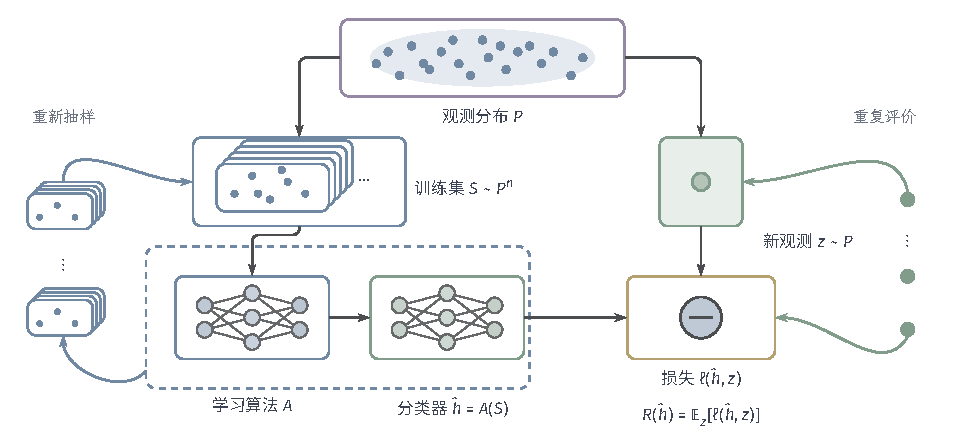
\includegraphics[width=164.600mm]{figures/03-foundations/02-learning-theory/tikz/learning-theory-two-randomness/figure.pdf}
  \caption{两层随机性的评价对象。固定训练模型后，右侧新观测的平均损失给出期望风险；左侧重新抽样则改变输出，学习保证控制这种变化造成高风险结果的概率。}
 \label{fig:learning-two-randomness}
\end{figure*}

\subsection{一般学习的风险与可学习性}
\label{sec:learning-problem-general-risk}

二分类例子已经给出两种平均：式~\eqref{eq:population-classification-risk}的总体平均和式~\eqref{eq:empirical-classification-risk}的样本平均。回归函数、聚类中心等决策也需要同样的两种平均，所以把它们写回第~\ref{sec:learning-problem-basic-setting}节的一般框架。二分类中的各个对象与一般框架的对应关系如下：

\begin{itemize}
\item 观测$z=(x,y)$是一封邮件的分数及其类别，观测空间$Z=X\times Y$；
\item 比较决策空间和输出决策空间都取假设空间$\mathcal H$（恰当学习），决策$w$就是分类器$h$；
\item 损失取零一损失$\ell(h,(x,y))=\ell_{01}(h(x),y)$；
\item 抽样机制取独立同分布，算法的内部随机性暂不考虑。
\end{itemize}

推广时，用一般观测$z$代替输入标签对，用决策$w$代替分类器$h$，损失由具体任务指定。被推广的只是风险的定义形式；“平均损失等于错误概率”这一解释只属于零一损失。

\begin{definition}[一般学习问题的期望风险]
\label{def:general-population-risk}
设$\mathcal P\in\mathfrak P$。对任意$w\in\mathcal W^+$，若$\ell(w,\cdot)$在$\mathcal P$下可积，则$w$的期望风险为
\[
 R_{\mathcal P}(w)=\mathbb E_{z\sim\mathcal P}\ell(w,z).
\]
\end{definition}

\begin{definition}[一般学习问题的经验风险]
\label{def:general-empirical-risk}
给定样本$S=(z_1,\ldots,z_n)\in Z^n$，任意$w\in\mathcal W\cup\mathcal W_{\mathrm{out}}$的经验风险为
\begin{equation}
 \hat R_S(w)=\frac1n\sum_{i=1}^n\ell(w,z_i).
 \label{eq:general-risk}
\end{equation}
\end{definition}

有了风险，就可以给“学习成功”定一个标准。这个标准需要回答四个问题，每个问题对应定义中的一个量。第一，和谁比？以比较决策空间中的最低期望风险$\inf_{w\in\mathcal W}R_{\mathcal P}(w)$为基准，即使这个基准不为零（空间里没有完美决策），也能衡量算法离最好的候选还有多远。第二，允许差多少？用容差$\varepsilon$限制输出风险比基准高出的部分。第三，有多大把握？训练样本是随机的，总可能抽到一份很不典型的样本，所以只要求成功的概率至少为$1-\delta$。第四，对哪些数据来源成立？算法不知道真实的$\mathcal P$，所以同一个算法、同一个样本量要求必须对$\mathfrak P$中的每个来源都有效。

\term{PAC学习}（probably approximately correct learning，概率近似正确学习）把这四点写在一起。名称里的“近似正确”对应$\varepsilon$允许的风险偏差，“概率”对应成功率至少为$1-\delta$。

\begin{definition}[相对于分布族的PAC可学习性]
\label{def:general-pac-learnability}
若存在算法$A$，对任意$\varepsilon,\delta\in(0,1)$存在整数$n_0(\varepsilon,\delta)$，使任意$\mathcal P\in\mathfrak P$和$n\geq n_0(\varepsilon,\delta)$均满足
\[
 \mathbb P_{S\sim\mathcal P^n,U}\!\left\{
 R_{\mathcal P}(A(S,U))\leq
 \inf_{w\in\mathcal W}R_{\mathcal P}(w)+\varepsilon
 \right\}\geq1-\delta,
\]
则称该学习问题相对于$\mathfrak P$是PAC可学习的。概率包含训练样本和算法内部随机数；确定性算法省略$U$。只有当$\mathfrak P$包含所讨论空间上的全部相关分布时，才称这一保证为分布无关。
\end{definition}

读这个定义时要注意量词的顺序：先有算法$A$，再给定容差$\varepsilon,\delta$，随后确定样本量门槛$n_0(\varepsilon,\delta)$，最后才对每个允许的来源$\mathcal P$提出要求。$n_0$只依赖两个容差，不能依赖$\mathcal P$；若允许先看到分布再定样本量，结论就只对那个分布成立，不再是对未知来源的保证。花括号里的事件说的是“这一次训练交出的决策，风险最多比基准高$\varepsilon$”，外层概率则对训练样本和内部随机数取平均。

为让这个不等式有意义，下文默认三个前提：类内风险下确界$\inf_{w\in\mathcal W}R_{\mathcal P}(w)$有限；算法输出的风险几乎处处有限；$R_{\mathcal P}(A(S,U))$作为$(S,U)$的函数可测，从而花括号中的事件有概率。零一损失下三者自动满足；对无界损失的具体定理，还要另用可积性或矩条件保证。这些前提只让PAC不等式写得出来，并不回答问题能不能学成。

定义~\ref{def:general-pac-learnability}还没有约束程序怎样执行，它只要求存在一个满足保证的映射。如果学习在给定编码下能停机、输出的预测程序对每个允许输入也都能停机，得到的是\term{可计算学习}（computable learning）；进一步要求样本量、训练时间和预测时间都有关于约定参数的多项式上界，才得到\term{高效学习}（efficient learning）。第~\ref{sec:pac-computation-requirements}节会在二分类中落实这两项附加要求。

\section{PAC学习}
\label{sec:pac-learning}

本节把定义~\ref{def:general-pac-learnability}落实到二分类：比较决策空间取为假设空间$\mathcal H$，损失取零一损失。先用一个具体数字体会两个容限。以可实现情形为例，要求“以至少99\%的概率，得到一个未来错误率不超过5\%的分类器”，就是取$\delta=0.01$、$\varepsilon=0.05$。其中5\%约束的是某一次训练得到的分类器在总体上的错误概率，99\%约束的是“抽一批样本再训练”这个随机过程成功的机会。这个要求既不要求训练集里每条记录都分对，也不要求每一批未来邮件的实际错误率都不超过5\%。

为什么要留出失败概率$\delta$？因为样本是随机抽取的，总可能恰好漏掉某些关键输入，所以只能允许小概率失败，再靠增加样本把失败概率压到$\delta$以下。至于“成功”时风险应当接近零，还是接近假设空间中最好的水平，取决于$\mathcal H$里是否存在零风险的假设。据此分出两种设定：可实现情形假设它存在，成功的基准是零风险；不可知情形不作这个假设，成功的基准是$\mathcal H$中的最低风险。两种设定使用同一套概率量词，只是允许的分布和风险基准不同。

\subsection{可实现情形}

先假设$\mathcal H$中确实存在一个在总体上零错误的假设。这个可实现条件暂时排除了标签噪声和假设空间表达不足造成的不可避免错误，让我们集中分析一个纯粹的问题：既然正确答案已经在假设空间里，有限的观测是否足以把它（或另一个风险同样低的假设）选出来。

\begin{definition}[可实现性]
\label{def:realizability}
如果某个假设能够以概率1正确预测数据来源中的标签，就称数据分布对该假设空间
是\term{可实现的}（realizable）。形式上，分布$\mathcal P$对$\mathcal H$可实现，
是指存在$h^\star\in\mathcal H$满足
\[
 R_{\mathcal P}(h^\star)=0.
\]
\end{definition}

前面的教学分布由阈值0.6确定真实标签，而$h_{0.6}$属于阈值空间，所以该分布是可实现的。要注意，要求的是总体中存在零风险的假设：如果同一个分数可以对应两种标签，分数本身就未必支持零错误预测；反过来，一张训练表上碰巧没有冲突标签，只说明有限观测没暴露矛盾，并不能据此确认可实现性。

但“存在零风险假设”既没有告诉算法该选哪一个，也没有告诉算法数据来自哪个分布。PAC因此要求算法和样本量都在看到数据之前确定：同一个算法、同一个样本量上界，必须对所有可实现分布都有效，样本量只能依赖$\varepsilon$、$\delta$和$\mathcal H$。如果先知道分布、再为它挑算法或定样本量，结论只适用于那一个特定分布，就不是PAC所要的统一保证。

把定义~\ref{def:general-pac-learnability}的允许分布族限定为所有对$\mathcal H$可实现的分布，并记样本量阈值为$m_{\mathcal H}$。此时类内最低风险为零，成功事件简化为
\begin{equation}
 \mathbb P_{S\sim\mathcal P^n}
 \left(R_{\mathcal P}(A(S))\leq\varepsilon\right)\geq1-\delta.
 \label{eq:pac-guarantee}
\end{equation}
这个式子要从内往外读。内层评价一次训练：$A(S)$是这次训练得到的分类器，$R_{\mathcal P}(A(S))\leq\varepsilon$是“这次成功”的事件，在零一损失下就是总体错误概率不超过$\varepsilon$。外层再对训练样本的随机抽取取概率，要求成功的概率至少为$1-\delta$。如果同一个算法对所有可实现分布都满足这一要求，就称$\mathcal H$是可实现PAC可学习的；$m_{\mathcal H}(\varepsilon,\delta)$可以依赖两个容限和假设空间，但不能随具体的未知分布改变。PAC这一计算形式化由Valiant提出，本章采用统计学习教材中的分布无关表述\scite{valiant1984}。

放回阈值例子，这个要求的含义很具体。在前面的教学分布下，真实分界是0.6，学到的阈值若为$\hat t$，错误就恰好发生在$\hat t$与0.6之间，风险等于分数落在这段区间的概率。于是$R_{\mathcal P}(A(S))\leq\varepsilon$说的是“学到的分界与真实分界之间只夹着概率不超过$\varepsilon$的邮件”。训练样本越多，0.6附近越可能出现训练点，把可选的阈值夹得越紧；但总有小概率抽到的邮件都远离0.6，这就是$\delta$要容许的失败。

PAC定义只要求存在某个够用的样本量，而实际关心的是“最少要多少”。满足要求的样本量门槛不止一个：若$n_0$够用，任何更大的数也够用。对给定的$\varepsilon$和$\delta$，在所有算法中，能使保证从某个样本量起一直成立的最小门槛，称为\term{样本复杂度}（sample complexity），它衡量这个学习问题本身需要多少数据。因此，证明某个$m_{\mathcal H}(\varepsilon,\delta)$满足要求，只给出了样本复杂度的一个上界；要说明不能更少，还需另外证明下界。

两个容限对应两种不同的改进方向：减小$\varepsilon$要求成功结果的风险更低，减小$\delta$要求训练失败更少；它们各自需要增加多少样本，要从假设空间和算法推导。第~\ref{chap:binary-learnability}章将在有限假设空间上具体计算这种样本量。

上面的保证允许指定任意小的精度，称为\term{强学习}（strong learning）。一个自然的问题是：如果手上只有一个“比瞎猜略好”的算法，能否把它加工成强学习算法？要讨论这个问题，先要把“比瞎猜略好”写准确。二分类中完全不看输入、按公平硬币猜测的错误率是$1/2$，只要求成功时的错误率比$1/2$低一个固定幅度，就得到\term{弱学习}（weak learning）。在可实现二分类中，它要求存在$\gamma\in(0,1/2)$、同一个算法$A$和有限的$m_{\mathcal H}^{\mathrm{weak}}(\delta)$，使任意$\delta\in(0,1)$、全部可实现分布$\mathcal P$及$n\geq m_{\mathcal H}^{\mathrm{weak}}(\delta)$都满足
\[
 \mathbb P_{S\sim\mathcal P^n,U}\!\left(
 R_{\mathcal P}(A(S,U))\leq\frac12-\gamma
 \right)\geq1-\delta,
\]
这时称$\mathcal H$弱PAC可学习。$\gamma$不随分布、样本或$\delta$变化，$U$独立于样本、表示算法的内部随机性，确定性算法省略它。取$\gamma=0.1$时，成功结果的错误率至多为40\%，比完全不看输入的公平猜测还低10个百分点。

定义中的关键是“统一”二字：优势$\gamma$对每个可实现分布都要成立。第~\ref{sec:boosting}节的提升方法正是借此把弱学习加工成强学习：它对样本重加权，在每一轮制造不同的分布，要求弱学习器在每一轮分布上都保持同样的优势，各轮的失败概率还要统一分配预算。因此，仅仅在一次训练上结果略优于猜测，并不能充当提升所要求的弱学习器。

\subsection{不可知情形}

如果假设空间里根本没有零风险的假设，可实现情形的前提就不成立。现实中这个前提往往无法确认，有时明知不成立。这时合理的做法是：先弄清在给定输入和假设空间下最低能达到多少风险，再看算法离这个最低水平有多远，而不能把“没达到零风险”直接算作学习失败。

零风险不可达有两种来源，必须分开。一是输入信息不足：即使完全知道分布，同一输入仍可能以正概率对应两种标签，这种错误不可避免。二是假设空间表达不了所需的预测关系，使$\mathcal H$内的最低风险高于所有可测分类器能达到的最低风险。第~\ref{sec:statistical-model-selection}节会分别用贝叶斯风险和近似误差刻画这两者。

无论是哪种来源，都不能再指望零风险，于是改用$\mathcal H$内的最低风险作为成功基准，并且不预先限制噪声的形式。这种设定称为\term{不可知设定}（agnostic setting）：它只要求学习结果接近这个基准，不承诺零风险的假设已经在$\mathcal H$内。“不可知”去掉的只是“假设空间内存在完美假设”这一项承诺；训练标签可用、样本独立同分布这两个条件仍然保留。

举个数字例子：假设$\mathcal H$的最低期望风险是8\%，那么要求恰当学习器达到2\%的总风险在这个空间里根本不可能；合理的要求是让它只比类内最低风险多2个百分点，即允许总风险达到10\%。学习输出的期望风险与类内最低风险之差称为\term{超额期望风险}（excess risk），它的参照始终是同一个$\mathcal H$，本例的容限就是2个百分点。

我们要比较的是“可以逼近的最低风险”，但空间中未必真的存在恰好达到它的成员，所以用下确界$R_{\mathcal P,\mathcal H}^\star$记录这个最佳逼近水平：
\begin{equation}
 R_{\mathcal P,\mathcal H}^\star=\inf_{h\in\mathcal H}R_{\mathcal P}(h).
 \label{eq:best-in-class-risk}
\end{equation}
例如假设空间中各假设的风险依次为$0.08+0.1/k$，可以无限趋近0.08却取不到它。用下确界就无需额外假设最优假设一定存在。

再把定义~\ref{def:general-pac-learnability}的允许分布族取为$X\times Y$上的全部相关联合分布，记充分样本阈值为$m_{\mathcal H}^{\mathrm{agn}}$，要求
\begin{equation}
 \mathbb P_{S\sim\mathcal P^n}\left(
 R_{\mathcal P}(A(S))\leq R_{\mathcal P,\mathcal H}^\star+\varepsilon
 \right)\geq1-\delta.
 \label{eq:agnostic-pac-guarantee}
\end{equation}
满足这一统一保证时，称$\mathcal H$是\term{不可知PAC可学习的}（agnostic PAC learnable）。注意容限$\varepsilon$限制的是超额期望风险，而不是全部风险。

可实现分布也包含在不可知保证覆盖的范围里：它的类内最低风险为零，式~\eqref{eq:agnostic-pac-guarantee}就退化为可实现保证。所以不可知学习扩大的是需要统一处理的分布范围，而不是放宽了成功标准。类内最低风险只用于评价，算法事先不需要知道它——这和可实现情形中算法不需要知道零风险假设具体是哪一个是同一个道理。

最后补充一点：“噪声”指什么，取决于评价时使用哪种标签。如果观测到的标签本身就是要预测的$y$，标签中的随机性就是分布$\mathcal P$的一部分，不可知设定已经把它包括在内；如果训练用的标签和评价用的标签不是同一种（例如用廉价标签训练、用专家标签评价），就要额外规定两种标签之间的关系，这时上面的同分布保证不能直接套用。

\subsection{计算要求}
\label{sec:pac-computation-requirements}

前面的PAC定义只把算法看成一个从样本到分类器的数学映射，回答的是“有限的信息是否足以可靠预测”。但存在这样一个映射，并不等于知道计算机怎样实现它：实现还要求训练和预测都真正能完成，并要核算计算量随问题规模怎样增长。为此在PAC的统计保证之上再加两层要求——可计算PAC要求程序能停机，高效PAC进一步要求资源有多项式上界；无论加哪一层，原来的统计保证都必须仍然成立。

核算之前先要固定编码：自然数输入写成二进制字符串，二分类标签占一个比特，假设由一个可计算的预测程序表示，学习器输出该程序的有限描述。任意实数未必有有限的精确编码，连续输入上的任意精度运算也要先约定精度或计算模型，不能默认把它当作一次常数时间操作计费。

\begin{definition}[可计算PAC学习]
\label{def:computable-pac-learning}
在固定的有效表示下，如果存在一个可执行的学习程序，能够在每个允许的有限训练样本上停机，输出一个对每个允许输入都能停机并给出标签的预测程序，并且该学习算法满足PAC保证，就称该假设空间是可计算PAC可学习的（computably PAC learnable），简称CPAC可学习。这里的PAC保证可以采用可实现版本或不可知版本，使用时必须说明采用哪一种。
\end{definition}

停机要求同时覆盖训练和使用两个环节。一句“返回期望风险最小的假设”并没有给出找到它的程序；输出一段可能永不返回的代码，也等于没有提供可用的预测规则。允许算法很慢、但最终能完成，就已经满足可计算性；多项式时间是在此之上的另一项要求。可计算PAC还按输出范围分两种：输出必须属于$\mathcal H$时称为恰当CPAC，允许输出$\mathcal H$之外的分类器时称为非恰当CPAC。本章默认恰当输出；引用文献结论时也要先确认对方使用的是哪一种输出约定，不能混用。

还要注意，训练可执行不代表能算出充分样本上界：前者只保证给定有限样本后训练能完成，后者要求算法能根据$\varepsilon,\delta$给出足够大的样本数。基本CPAC不自动要求后者，附加可计算样本上界的版本及相关分离结果见Delle Rose等人的工作\scite{dellerose2023}，第~\ref{sec:computable-binary-learning}节会用可计算的缺失标记来说明这项区别。

有限个假设可以穷举，但穷举可能需要指数时间。设假设由$d$个比特索引，共有$2^d$个成员、每个都能在多项式时间内求值，那么逐一计算经验风险仍要检查指数多个候选。而定理~\ref{thm:finite-realizable-pac}给出的可实现充分样本量只按
\[
 \frac{d\log2+\log(1/\delta)}{\varepsilon}
\]
增长。样本量上的线性和穷举规模上的指数并不矛盾，它们衡量的是两种不同成本：前者是信息成本（需要多少数据），后者是搜索成本（找到好假设要多少计算）。这个比较只说明穷举不够高效，并没有排除利用结构设计更快算法的可能。

\begin{definition}[高效PAC学习]
\label{def:efficient-pac-learning}
高效PAC学习（efficient PAC learning）要求在满足PAC期望风险保证的同时，样本量、训练计算量及输出分类器的预测计算量都有多项式上界。为明确规模依赖，考虑由参数$d$描述的一族假设空间$\mathcal H_d$，并约定观测编码长度上界为$b$。本书采用的高效性约定要求存在统一程序和固定多项式$p,q$，使所需样本量及训练时间分别满足
\begin{equation}
 \begin{aligned}
 m_{\mathcal H_d}(\varepsilon,\delta)
 &\leq p\bigl(d,b,1/\varepsilon,\log(1/\delta)\bigr),\\
 T_{\mathrm{train}}
 &\leq q\bigl(n,d,b,1/\varepsilon,\log(1/\delta)\bigr).
 \end{aligned}
 \label{eq:efficient-pac-resources}
\end{equation}
学习程序把$d,\varepsilon,\delta$及样本编码作为输入；若$\varepsilon,\delta$只通过预先给定的
样本量体现，也必须明确这一接口。输出分类器属于预先规定、可统一求值的表示族，它在新的预测输入
上的求值时间应被$d$、输出表示长度和输入编码长度的某个固定多项式所控制，不能仅把任意
程序的短代码长度当作预测高效的依据。若这族假设空间还由目标描述长度等量参数化，也须将
它们明确列入规模变量。
\end{definition}

以多项式作为“高效”的界线，是计算复杂性理论的通行约定：多项式增长在规模加倍时只让成本乘上一个固定倍数，指数增长则让成本随规模每增加一点就成倍膨胀；这条界线还不随编码细节的合理变化而改变。规模参数$d$由具体问题约定，不一定是特征维数；编码长度$b$则保证长数值的读写和比较都计入成本。统一多项式还要求次数不随$d$增长。不同文献有时用$1/\delta$、有时用$\log(1/\delta)$描述资源，引用时必须核对。即使满足多项式上界，很大的常数或很高的次数也可能让实际计算难以承受。

穷举是最坏的做法，问题若有结构，搜索可以快得多。阈值空间就是一例。设输入是$1,\ldots,M$中的整数，假设为$h_t(x)=\mathbb I\{x\geq t\}$，$t\in\{1,\ldots,M+1\}$，其中$\mathbb I\{\cdot\}$在括号内条件成立时取1、否则取0。候选有$M+1$个，而$M$的编码只占约$\log M$位，逐个检查对编码长度而言是指数代价。关键观察是：阈值在两个相邻的已见输入之间移动时，样本上的预测不变，只有越过某个已见输入时才会改变，所以只需检查至多$n+1$个切分位置。

具体做法分三步。先把样本按输入排序、合并重复输入，记下每个输入处正、负标签各有多少。再从左到右扫描每个切分位置：切分左侧的正标签被判为负，右侧的负标签被判为正，二者之和就是该切分的训练错误数，每移动一个位置只需增减一次计数。最后选错误最少的切分。排序需要$O(n\log n)$次比较，扫描需要$O(n)$次累计；比较一次输入约需$\log(M+1)$位，计数约需$\log(n+1)$位；预测只需一次阈值比较。结合有限假设空间的样本界，这个算法在所述编码下满足高效PAC的要求。

固定风险目标、表示方式和输出范围后，三层要求之间有包含关系：满足高效PAC一定满足可计算PAC，满足可计算PAC一定满足定义~\ref{def:general-pac-learnability}的统计意义上的PAC；反方向都需要补充条件。本节出现的几组概念限制的是学习的不同侧面：可实现与不可知限制数据分布，恰当与非恰当限制输出范围，可计算与高效限制执行方式。它们可以组合使用，但不能用其中一项代替另一项。

\section{学习的限制}
\label{sec:limits-of-learning}

第~\ref{sec:pac-learning}节规定了什么叫学习成功，但没有说明算法应当怎样从样本中选出假设。面对未知的$\mathcal P$，算法算不出期望风险，却能逐条算出训练损失，于是“选训练平均损失最小的假设”成了最自然的做法。前面的阈值0.4和0.6在四封邮件上都是零错误，按这个做法都可能被选中。本节说明这种做法本身为什么不足以保证学习成功，以及更根本地，为什么任何算法都需要对假设空间加以限制。

\begin{definition}[经验风险最小化]
\label{def:erm-learning-rule}
\term{经验风险最小化}（empirical risk minimization, ERM）是在给定假设空间中，选择
训练样本平均损失最小的假设作为学习结果。用$A_{\mathrm{ERM}}$表示这种学习算法，则
\begin{equation}
 A_{\mathrm{ERM}}(S)\in\argmin_{h\in\mathcal H}\hat R_S(h).
 \label{eq:erm-learning-rule}
\end{equation}
这里$\argmin$表示所有达到最小经验风险的假设组成的集合。若最小值不能取得，可以
要求输出的经验风险与下确界相差不超过一个给定容差。
\end{definition}

$\argmin$可能包含多个假设，式中的“$\in$”表示算法可以任选其中一个，也就是说ERM本身没有规定出现并列时选哪一个。阈值0.4和0.6就是这样一对并列的经验最优解：训练风险相同，对未见输入的预测却不同。这说明从“训练风险最小”推不出“总体风险小”，要得到PAC式的成功，还必须另外控制那些没有被样本观察到的区域上的风险。

增加样本也未必能消除这个问题：如果假设空间里允许“把这份样本逐条记下来”的规则，新增数据只会让记下来的表更长。下面构造一个具体例子，检验零训练错误能否单独推出低期望风险。

\subsection{记忆训练样本}

仍以$[0,1]$上的邮件分数为输入，这次假设分数均匀分布（某个区间的概率就等于它的长度），并且所有真实标签都是垃圾邮件。这是一个人为简化的分布，便于直接计算“推广”和“记忆”两种规则的风险。

在这个分布上，“始终预测垃圾邮件”的规则一次都不会错。再考虑另一种规则：它把训练中出现过的分数记在一张表里，分数在表中就预测垃圾邮件，不在表中就预测正常邮件。两种规则都能分对全部训练邮件，但对表外的输入，预测结果正好相反。

将记忆表写成有限分数集合$C$，规则为
\begin{equation}
  h_C(x)=
  \begin{cases}
    1, & x\in C,\\
    0, & x\notin C,
  \end{cases}
  \label{eq:finite-memory-classifier}
\end{equation}
再令$h_{\mathrm{all}}(x)=1$，把它和所有有限表规则$h_C$一起放入假设空间。这些规则都可测，而且$h_{\mathrm{all}}$的总体风险为零，所以这个分布对该假设空间是可实现的。（技术上，这个反例只在一个固定分布上计算两个具体输出的风险，不需要对整个假设空间取上确界，所以用不到第~\ref{sec:learning-problem-basic-setting}节末尾的可数逼近约定；下面按样本选出的$h_{C_S}$及其风险都是可测的。）

用$C_S$记录样本$S$中出现过的全部不同输入。选择$h_{C_S}$是一个合法的零经验风险选解，但它的两项风险分别为
\begin{equation}
  \hat R_S(h_{C_S})=0,
  \qquad
  R_{\mathcal P}(h_{C_S})=1.
  \label{eq:memorization-erm-failure}
\end{equation}
每个训练点都在表内，所以经验风险为零；连续均匀分布落在任意有限集合上的概率为零，所以新输入几乎必在表外，总体风险为1。零训练错误和几乎处处预测错误，在同一条规则上同时成立。

要注意，如果ERM在并列时总是选$h_{\mathrm{all}}$，它在这个例子里就成功了。所以反例说明的不是“ERM必然失败”，而是“训练风险最小”这个要求本身约束不住最终选出哪个假设：它只管已见点上的损失，对表外的输入怎样回答完全不加限制。第~\ref{sec:binary-uniform-convergence}节将用一致收敛把经验风险和总体风险连接起来，从而保证所有经验最优解都接近类内最低期望风险。

\subsection{没有免费的午餐}
\label{sec:no-free-lunch}

记忆规则的失败引出一个更一般的问题：如果不用ERM，换一种更聪明的选择方法，能不能对任意标签规律都保证成功？答案是否定的。只要假设空间允许许多输入的标签彼此毫无约束地变化，已见标签就提供不了任何关于未见标签的信息。\term{没有免费的午餐}（no-free-lunch）定理把这个信息缺口写成一个对任意有限样本算法都成立的失败下界。它的名字说的正是这个意思：不利用问题本身的结构，就不存在在所有情形下都保证成功的通用方法。

先看定理要证明什么。设算法只能看到$n$个观测，而假设空间能在某$2n$个输入上实现全部可能的二元标签组合。那么无论算法是什么，都能找到一个分布，它在$\mathcal H$中有零风险的假设，但算法仍以至少$1/7$的概率得到期望风险不低于$1/8$的结果。直觉是：$n$个观测最多覆盖$2n$个输入中的一半，另一半的标签可以任意设定，而这些标签不受已见标签任何约束，算法在那里只能碰运气。注意这里的“失败”指总体风险超过容限，训练错误完全可以是零。

先用四个输入看清这种歧义，再给出一般证明。令$X=\{1,2,3,4\}$、四者等概率出现，编号只用来区分对象，不携带类别或相似性信息；假设空间允许全部二分类函数。若训练只出现$(1,0)$和$(2,1)$，编号3、4的标签仍然未知。

把完整标签表$(0,1,0,0)$和$(0,1,1,1)$分别记为$f_0$、$f_1$。它们在训练点上完全相同，都解释已见标签，在编号3、4上却处处相反。所以“与样本一致”只代表在观察到的点上回答正确。图~\ref{fig:learning-no-free-lunch}并列画出这两套隐藏真值。

\begin{figure*}[!htb]
  \centering
  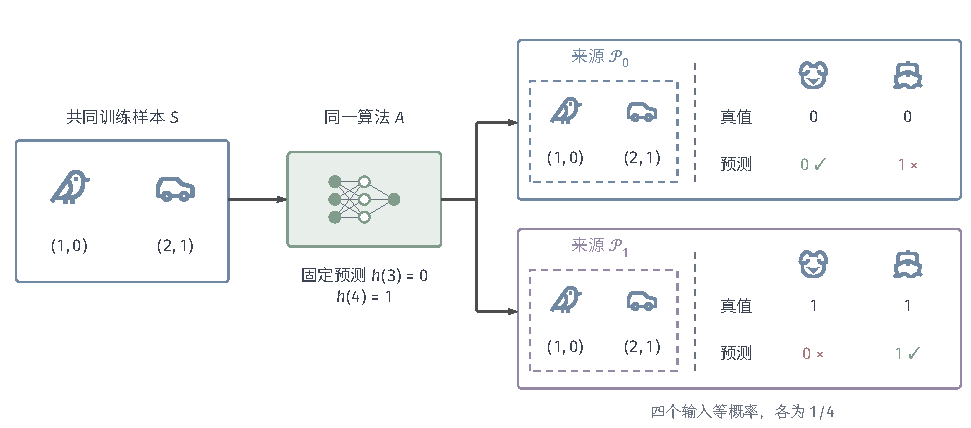
\includegraphics[width=164.600mm]{figures/03-foundations/02-learning-theory/tikz/learning-theory-no-free-lunch/figure.pdf}
  \caption{相同样本与两套隐藏标签。鸟、汽车、狗、船分别表示编号1至4，每个概率为$1/4$；两套来源在已见编号1、2上同为0、1，未见编号3、4则分别全为0或全为1。图示输出$h(3)=0,h(4)=1$在每套来源各错一个点。固定样本与内部随机数后输出相同，任意二元预测在每个未见点的两份损失相加为1，故风险之和至少$1/2$。这里展示固定样本的歧义，下文再证明随机抽样下的固定困难分布。}
 \label{fig:learning-no-free-lunch}
\end{figure*}

预测编号3时，$f_0$要求回答0，$f_1$要求回答1。两套真值交给算法的样本都是$(1,0),(2,1)$，算法无法凭这份样本辨认当前面对的是哪一套；它可以按某种偏好选一个标签，但这个偏好同样可能与真实标签相反。

即使把所有假设枚举一遍，也只能发现$f_0$和$f_1$的训练错误都为零：枚举只是列出了所有假设，却没有提供“二者在编号3上谁对”的证据。要消除歧义，只能直接观察该标签，或者在已见标签与未见标签之间加入某种联系。

把同样的歧义放到$2n$个等概率输入上。给定$n$个观测，未见输入组成的集合$V$至少包含$n$个点；当两张标签表在已见处相同、在$V$上处处相反时，同一个输出$h$在每个未见点上的两份零一损失相加恰好为1，因此
\[
 R_{\mathcal P_0}(h)+R_{\mathcal P_1}(h)
 \geq\frac{|V|}{2n}\geq\frac12.
\]
所以两张表中至少有一张，会使这次输出的风险不低于$1/4$。但这个论证是“先看到样本、再拿两张标签表对照”，而定理要求困难分布在抽样之前就已经确定——量词顺序必须是“先固定算法和样本量，再存在一个分布”。为此，证明改为对所有可能的标签表取平均，再从中挑出一个固定的分布\scite{shalevshwartz2014}。

\begin{theorem}[没有免费的午餐]
\label{thm:no-free-lunch-classification}
设$n\geq1$，固定预测输入空间$X$中有一个含$2n$个不同点的集合$C$。假设无论怎样为
$C$中的每个点分别指定标签0或1，都能从$\mathcal H$中找到一个分类器，使它在$C$上的
预测与这些指定标签完全一致；不同的标签组合可以由$\mathcal H$中的不同分类器实现。
则对任意使用$n$个独立同分布训练观测的二分类学习算法$A$，都存在一个对$\mathcal H$
可实现的分布$\mathcal P$及$f^\star\in\mathcal H$，使$R_{\mathcal P}(f^\star)=0$，但
\begin{equation}
 \mathbb P\left(R_{\mathcal P}(A(S))\geq\frac18\right)\geq\frac17.
 \label{eq:no-free-lunch-probability}
\end{equation}
这里概率对$S\sim\mathcal P^n$及算法内部随机性计算。算法即使允许输出$\mathcal H$以外的分类器，结论也成立。
\end{theorem}

\begin{proof}
固定输入集合$C$并让输入均匀出现，不同的分布之间只有标签表不同。对任意$g:C\to\{0,1\}$，前提给出$f_g\in\mathcal H$与它在$C$上一致。按先抽输入、再取标签$g(x)$的方式定义$\mathcal P_g$，这个分布就由$f_g$实现，风险为零。

暂时给$C$中每个输入独立分配一个公平的二元标签，用来对所有可能的标签表取平均。每个点只分配一次，重复抽到它时标签保持不变。因此任意固定标签表仍对应无噪声的可实现分布；随机标签表是证明工具，不是训练过程中不断变化的真值。

固定训练输入、已见标签与算法随机数后，算法输出也已确定。$n$个观测至多涉及$n$个不同输入，故$C$中至少$n$个输入未见。每个未见标签仍是独立公平的二元选择，无论输出在该点回答0还是1，条件错误概率都是$1/2$。

输出$h$在$\mathcal P_g$下的风险，是$C$中$h$答错的点所占的概率之和，每个点的概率为$1/(2n)$。已见点上的错误只会使风险更大，因此只累加未见点，就得到一个下界。对随机标签表取条件期望，每个未见点贡献$1/(2n)\times1/2$，至少$n$个未见点合计为
\begin{equation}
 n\times\frac1{2n}\times\frac12=\frac14.
 \label{eq:no-free-lunch-expected-risk}
\end{equation}
三个因子依次为未见点数下界、单点概率与条件错误概率。这个下界对每一种训练输入、已见标签和内部随机数都成立，所以再对它们取平均仍不低于$1/4$。交换平均的次序（先固定标签表$g$，再对$\mathcal P_g$下的样本$S$及内部随机数$U$平均），得到$\mathbb E_g\mathbb E_{S,U}R_{\mathcal P_g}(A(S,U))\geq1/4$。

标签表只有有限张，平均至少为$1/4$就必有固定$g^\star$满足
\[
 \mathbb E_{S,U}R_{\mathcal P_{g^\star}}(A(S,U))\geq\frac14.
\]
若每张表的平均风险都小于$1/4$，总平均也会小于它，产生矛盾。现在固定$\mathcal P=\mathcal P_{g^\star}$及$f^\star=f_{g^\star}$，后续概率只包含从这个固定来源抽样与算法随机性。

最后把平均风险下界转成失败概率。思路是：风险最多为1，若风险很少超过$1/8$，平均就不可能达到$1/4$。令$Q=R_{\mathcal P}(A(S,U))\in[0,1]$、$p=\mathbb P(Q\geq1/8)$。失败事件外$Q<1/8$，事件内$Q\leq1$，从而
\[
 \frac14\leq\mathbb E Q\leq(1-p)\frac18+p
 =\frac18+\frac78p.
\]
移项即得$p\geq1/7$。\end{proof}

要特别注意困难分布的选择时机：它是在算法$A$和样本量$n$固定之后才选出的；此后所有重复训练都从这同一个分布抽样，输入频率和标签表不再改变，算法以至少$1/7$的概率得到风险不低于$1/8$的输出。证明并没有在看到某次具体样本后再去修改标签，所以它给出的是固定来源上的随机训练失败，而不是事后挑出一批不利样本。

还要看清定理的适用范围。困难分布可以随$A$和$n$变化，因为定理是针对每个算法、每个样本量分别构造反例的：它既不要求同一个分布能击败所有算法，也没有说某个算法在所有分布上都失败。面对有结构的数据，算法完全可能成功；被排除的只是“在标签可以任意设定的所有分布上都统一成功”。

这个有限样本结论可以推出一个关于无限空间的结论。设$X=\mathbb N$，$\mathcal H$包含全部二分类函数，并假设它PAC可学习。取$\varepsilon=1/16$、$\delta=1/8$，按定义就存在一个有限的样本量$n$，对所有分布都保证成功。但从$X$中任选$2n$个点，定理都能构造出一个可实现分布，使算法以至少$1/7>\delta$的概率得到风险至少$1/8>\varepsilon$的结果，与假设矛盾。所以这个不受限制的假设空间不是PAC可学习的。要注意，不能被统一学习的是整个空间，而不是其中的每一个具体分布。

这里的可实现性只保证正确的完整标签表$f^\star$属于$\mathcal H$，并没有把这张表交给学习器。学习器只看到$n$条带标签记录；把某个未出现编号的标签改成另一类、其余保持不变，就得到另一张同样能解释全部样本的表。所以“零风险的假设存在”和“样本足以确定它在未见点上的预测”是两个不同的条件，前者成立并不意味着后者成立。

这也说明这里的失败不是搜索时间不够：即使允许无限计算，算法看到的仍是同一份样本和彼此冲突的可能真值表，无法靠搜索判断哪张表才是真实来源。第~\ref{sec:pac-computation-requirements}节讨论的不可计算或时间过长限制的是执行；这里的限制来自标签信息本身的缺失。

有人可能会想：PAC的要求已经很弱了，它不要求复原整张真值表，只要求总体风险低于$\varepsilon$，也许能绕开这个困难。但上面的下界恰恰是针对这个较弱的要求证明的：对任何有限的样本量，都存在可实现分布让它以过大的概率失败。所以即使只要求低风险，也无法为不受限制的假设空间找到统一的有限样本量。

要有正面保证，就必须让一个标签能够约束其他输入上的预测。例如阈值规则一旦在分数0.5、标签为1的邮件上分对，就必有$t\leq0.5$，于是所有更高分数也被预测为1：观察一个标签就排除了许多阈值，从而限制了未见预测。反过来，如果每个编号的标签都可以自由选择，编号1的标签对编号2就不提供任何信息。

限制假设空间或限制分布族，正是在加入这种可以推广的联系；而限制也有代价：如果真实规律不满足它，真正需要的假设反而会被排除。下一节就在同一个风险口径下分析这种表达代价，以及有限样本带来的选择代价。

\section{风险来源与模型选择}
\label{sec:statistical-model-selection}

第~\ref{sec:limits-of-learning}节说明必须限制假设空间，本节分析这种限制的代价，以及怎样在限制强弱之间作出选择。先看一个例子：如果垃圾邮件的分数集中在两个分离的区间、中间反而是正常邮件，单个阈值就不可能同时圈住两段垃圾邮件而排除中间的正常邮件。阈值这一限制减少了预测的自由度，但也留下了再多训练样本都消除不了的误差。要合理选择假设空间，先要把这种“假设空间不够用”的误差，和“输入信息本身不够”的误差区分开。

先看输入信息不足。设分数0.5的邮件中有70\%是垃圾邮件、30\%是正常邮件，而分类器只能看到$x=0.5$，于是对这类邮件只能给出同一个预测：预测垃圾邮件会错30\%，预测正常邮件会错70\%，任何分类函数在这个输入上的条件错误率都不可能低于30\%。只要表示仍是这个单一分数，更多样本或换一个算法都无法区分这些邮件。

空间限制是另一种情形。设三个输入分数为0.2、0.5、0.8，标签分别确定为1、0、1：输入足以区分三者，也存在把它们全部分对的函数，但单阈值产生不了“1、0、1”的变化，任何阈值都至少错一类。这里缺的不是区分输入的信息，而是$\mathcal H$中能利用这些信息的规则。

这两个例子提示我们分两步确定比较基准：先求在当前输入信息下，所有可能的分类器最低能达到多少风险；再看把分类器限制在$\mathcal H$内之后，这个最低值被抬高了多少。前者称为贝叶斯风险，后者衡量假设空间的表达限制。

\term{贝叶斯风险}（Bayes risk）是在当前输入信息下、所有可测分类器能达到的最低错误概率。达到它的规则叫贝叶斯决策：对每个输入，选择在给定该输入时期望损失最小的预测（这需要条件风险有限、最小值能取到且选择规则可测；一般损失下的决策概念可参考\BookVolumeRef{vol:mathematical-preliminaries-lower}{卷2《数学准备：概率、因果与决策》}）。这里用二分类零一损失。令$\mathcal H_{\mathrm{all}}$为全部可测二分类器，贝叶斯风险写成
\begin{equation}
 R_{\mathcal P}^\star=\inf_{h\in\mathcal H_{\mathrm{all}}}R_{\mathcal P}(h).
 \label{eq:bayes-risk}
\end{equation}
这个基准不要求分类器属于所选的$\mathcal H$，它描述的是“完全知道数据规律时”能达到的水平；它只是评价的参照，并不假定学习器知道它。

计算贝叶斯风险可以逐个输入来做：先在一个输入$x$处比较两种预测的错误率，再对所有输入取平均。为此需要知道给定输入时标签的条件概率。把联合分布中的标签忽略掉，得到输入自身的分布，记为$\mathcal P_X$。给定$x$时标签为1的条件概率记为
\[
 \eta(x)=\mathbb P(y=1\mid x),
\]
相应地，标签为0的条件概率是$1-\eta(x)$。（技术上，条件概率只在$\mathcal P_X$几乎处处意义下唯一；本章的实数区间和欧氏向量输入都满足所需的正则性，不同版本只在概率为零的输入集合上不同，不影响总体风险。）

在$x$处预测1，错误概率是$1-\eta(x)$；预测0，错误概率是$\eta(x)$。两者取其小，就应在$\eta(x)\geq1/2$时预测1，否则预测0，相等时两种预测都最优。逐点这样选择得到\term{贝叶斯分类器}（Bayes classifier）：
\[
 h^\star(x)=\mathbb I\{\eta(x)\geq1/2\}.
\]
于是每个输入处的最小条件错误率为
\[
 \min\{\eta(x),1-\eta(x)\}.
\]

在分数0.5处，$\eta(0.5)=0.7$意味着两种预测的条件错误率分别为0.3和0.7；贝叶斯分类器选择预测垃圾邮件，但仍会把其余30\%的正常邮件分错。这个例子把“选多数标签”的规则与“只观察分数时不可避免的错误”联系了起来。

逐点的条件错误率还要按输入出现的频率加权，才得到总体风险。例如分数0.5的邮件占全部邮件的比例为$q$，它对总体错误的贡献就是$0.3q$。用输入的\term{边缘分布}（marginal distribution）$\mathcal P_X$平均上述逐点最小值：
\[
 R_{\mathcal P}^\star=
 \mathbb E_{x\sim\mathcal P_X}[\min\{\eta(x),1-\eta(x)\}].
\]
如果存在一个正$\mathcal P_X$测度的输入集合，其中两类标签都有正的条件概率，这个平均就严格为正：即使完全知道分布、采用贝叶斯规则，当前输入本身仍会留下无法消除的错误。

\subsection{两类误差}

有了贝叶斯风险这个最低基准，就可以把学习结果多出来的风险拆成两段：第一段是因为把分类器限制在$\mathcal H$内而抬高的最低风险，第二段是算法在$\mathcal H$内的实际选择偏离$\mathcal H$内最低风险的部分。

第一段称为\term{近似误差}（approximation error），等于类内最低期望风险减去贝叶斯风险。固定评价分布、输入表示和损失之后，它刻画假设空间的表达限制；在这些对象不变时，即使拥有无限数据、并能找到类内最优的假设，也消不掉这段差距。

第二段通常称为\term{估计误差}（estimation error），等于输出的期望风险减去类内最低期望风险。对一般算法，更准确的称呼是\emph{类内超额风险}，因为这段差距里未必只有统计波动：优化没有真正收敛、正则化改变了优化目标、并列解的选择方式不一致，都可能贡献其中一部分。

对恰当输出$\hat h=A(S)\in\mathcal H$，在贝叶斯风险和输出风险之间插入类内下确界，就得到两段分解：
\begin{align}
 R_{\mathcal P}(\hat h)-R_{\mathcal P}^\star
 ={}&\left(\inf_{h\in\mathcal H}R_{\mathcal P}(h)-R_{\mathcal P}^\star\right)
 \label{eq:approximation-estimation-decomposition}\\
 &+\left(R_{\mathcal P}(\hat h)-\inf_{h\in\mathcal H}R_{\mathcal P}(h)\right).
 \notag
\end{align}
第一项是近似误差，第二项是估计误差。$\mathcal H\subseteq\mathcal H_{\mathrm{all}}$保证第一项非负，$\hat h\in\mathcal H$保证第二项非负；如果允许输出比较空间$\mathcal H$之外、但仍在算法输出空间$\mathcal W_{\mathrm{out}}$内的结果，它可能优于$\mathcal H$的下确界，第二项就可能为负，这时非负分解的解释也要相应改变。

用一个教学数字串起这三个水平：贝叶斯风险5\%，阈值空间的最低风险12\%，学到的阈值风险15\%。那么表达限制贡献7个百分点，类内选择贡献3个百分点，输出总共高于贝叶斯风险10个百分点。扩大假设空间可以降低第一段的近似误差，但如果同时改变了输入表示，全部可测分类器的贝叶斯基准和新的候选空间都要重新定义，原来的5\%、12\%和7个百分点不能原样沿用。

两段差距对数据量的反应不同。近似误差在空间固定时与样本量无关；第二段则有可能随样本增多而缩小，但这取决于算法。始终返回同一个坏假设的算法，样本再多也不会改善。描述“样本越多、第二段越小”这一性质的术语是\term{一致性}（consistency）：对每个固定的允许分布，样本量趋于无穷时，类内超额风险依概率趋于零，也就是对任意固定的正容差，超额风险超过它的概率趋于零。这里的“一致”既不是指标签彼此一致，也不是指某次优化已经收敛。它与PAC可学习的区别在于样本量是否统一：一致性允许所需样本量随分布变化，PAC要求一个对所有允许分布都够用的样本量；几乎处处收敛、期望收敛等其他版本也须分别说明。还要注意，只有当泛化偏差和近似求解的容差都得到控制时，ERM或近似ERM的超额风险上界才能主要解释为有限样本带来的统计代价，而不混入优化不充分等因素。

图~\ref{fig:approximation-estimation-error}沿风险增大的方向排列这三个水平：贝叶斯风险到类内最低风险的距离是近似误差，类内最低风险到输出风险的距离是估计误差。后一段距离的具体来源仍取决于算法，只有结合ERM、近似ERM或其他一致性保证，才能把它的上界解释为有限样本代价。

\begin{figure}[htbp]
  \centering
  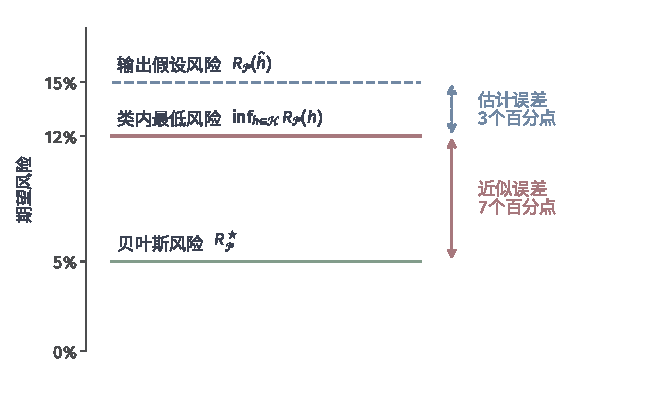
\includegraphics[width=112.000mm]{figures/03-foundations/02-learning-theory/matplotlib/learning-theory-error-decomposition/figure.pdf}
  \caption{风险的两段差距。教学设定中，贝叶斯风险为5\%，阈值空间最低风险为12\%，输出风险为15\%。前两者相差7个百分点，为实线表示的近似误差；后两者相差3个百分点，为虚线表示的估计误差。}
  \label{fig:approximation-estimation-error}
\end{figure}

扩大假设空间一方面提供了更多逼近目标的机会，另一方面也提供了更多偶然拟合样本的机会。\term{偏差与复杂度的权衡}（bias--complexity trade-off）说的就是这个选择：这里的“偏差”指空间的表达限制，“复杂度”指在有限样本中可靠选解的统计代价。

如果正类由两个分离区间组成，单阈值的近似误差不会因数据无限增加而消失；允许许多小区间的并以后，空间既能表达这种正类，也能把训练点紧密包围起来，未见的间隙反而可能被误判，类内选择的统计误差更难控制。式~\eqref{eq:approximation-estimation-decomposition}的两段随空间一起变化，最终风险未必下降。结构风险最小化正是用来比较“拟合收益是否足以补偿新增的不确定性”。

算法对训练目标本身的求解差距还要单独列出。如果$\mathcal H$中训练错误最少的假设只错2封、算法返回的假设错5封，多出来的3次错误来自经验目标没有真正最小化。\term{经验优化误差}（empirical optimization error）用两个经验风险之差计量：
\begin{equation}
  \Delta_{\mathrm{opt}}(S)
  =\hat R_S(\hat h)-\inf_{h\in\mathcal H}\hat R_S(h)
  \geq0,
  \label{eq:empirical-optimization-error}
\end{equation}
要注意，经验优化误差比较的是样本上的目标值，而式~\eqref{eq:approximation-estimation-decomposition}的两项都是总体期望风险，两者不是一回事，不能把那个两项恒等式直接改写成三个非负的期望风险之差。正确的顺序是先建立泛化控制、把经验量和总体量连接起来，再把$\Delta_{\mathrm{opt}}(S)$纳入输出风险的保证。

\subsection{用验证样本选择模型}
\label{sec:validation-model-selection}

如果嵌套的假设空间逐渐扩大、每次又都精确最小化经验风险，训练误差只会持平或下降。但这种下降本身无法判断未来误差的走势：更大的空间总能把训练样本拟合得一样好或更好，包括拟合其中的偶然性。要比较不同复杂度或其他超参数，就需要一批不参与参数拟合的\term{验证样本}（验证样本为什么不能再当测试用，见第~\ref{sec:experience-data-boundary}节）。若验证样本独立于训练过程、且与未来数据同分布，那么对某个固定模型，验证误差是未来误差的无偏估计；但选择本身会引入偏差。设有20个候选的真实错误率都是10\%，各自的验证误差围绕10\%随机波动，挑出其中最小的那个，它的验证误差通常低于10\%，这种偏低并不代表该模型更好。候选越多，偶然偏低的机会越大，因此最终评价必须覆盖“调参并选择模型”的整个流程，而不只是选中之后的模型（多次比较的统计含义可参考\BookVolumeRef{vol:mathematical-preliminaries-lower}{卷2《数学准备：概率、因果与决策》}）。

图~\ref{fig:learning-model-selection}用教学曲线展示这种背离：训练误差持续下降时，验证误差可能转而回升，合适的复杂度由验证误差的最低点确定，实际曲线也未必只有一个谷底。由于验证样本已经参与选择，锁定模型和超参数之后，还要再用独立的\term{测试样本}评价最终结果；如果继续看着测试误差改模型，测试样本也参与了选择，这次“独立评价”就失去了意义。

\begin{figure}[htbp]
  \centering
  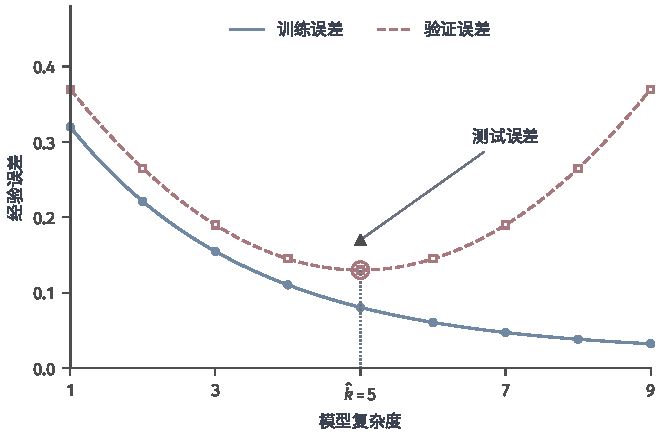
\includegraphics[width=112.000mm]{figures/03-foundations/02-learning-theory/matplotlib/learning-theory-model-selection/figure.pdf}
  \caption{教学示意中的验证选择与独立测试。实线圆点为训练误差，虚线方块为验证误差，圆环的最低验证误差确定$\hat k$。三角形仅为锁定模型后的一次测试评价，未参与选择，故不连成测试曲线。所有数值均为构造示意。}
 \label{fig:learning-model-selection}
\end{figure}

\subsection{结构风险最小化}

把假设空间写成一列嵌套集合$\mathcal H_1\subseteq\mathcal H_2\subseteq\cdots$，例如让$\mathcal H_k$允许至多$k$个区间的并作为正类区域。单纯比较最小经验风险会偏向更丰富的空间，因为它至少保留了前一个空间的全部候选；但只选最简单的空间又可能留下较大的近似误差。我们需要一条规则，同时顾及表达限制和有限样本下的选择代价。

验证选择和SRM都在解决“看过数据后再选模型”的偏差，但依据的证据不同：验证选择是另留一批数据直接估计各个模型的表现；\term{结构风险最小化}（structural risk minimization, SRM）不另留数据，而是在同一批训练样本上，用对所有候选空间同时成立的理论偏差上界构造一个复杂度惩罚，二者不能互相等同。

为什么要靠惩罚而不是直接最小化风险？因为近似误差和估计误差都依赖未知分布、无法直接计算，能计算的只有经验风险，所以在经验项之外加上一个随复杂度增长的惩罚，作为统计不确定性的抵扣。具体做法是先固定总失败预算$\delta$，再给每个空间分配一个与样本无关的预算$\delta_k>0$、满足$\sum_{k\geq1}\delta_k\leq\delta$；用$\operatorname{pen}(k,n,\delta_k)$记录第$k$个空间的复杂度惩罚，然后选择
\begin{equation}
  (\hat k,\hat h)
  \in\argmin_{k\geq1,\,h\in\mathcal H_k}
  \left\{\hat R_S(h)+\operatorname{pen}(k,n,\delta_k)\right\}.
  \label{eq:structural-risk-minimization}
\end{equation}
经验项衡量训练拟合的好坏，惩罚控制由样本推断总体时的不确定性，通常随空间复杂度增大。它是控制估计误差的工具，而不是估计误差本身：惩罚太小可能选中偶然拟合的复杂规则，太大又可能留下简单空间的表达偏差。最小值不可达时，可以取带惩罚目标的近似最优解。

同时比较多个空间，需要的是“同时有效”的偏差保证。每个空间单独的失败概率都不超过$\delta$，并不能保证看过数据再从中选一个之后总失败概率仍不超过$\delta$；预先分配$\delta_k$并令$\sum_k\delta_k\leq\delta$后，并集界就控制了“至少一个空间估计失准”的概率，从而以至少$1-\delta$的概率，所有空间同时满足各自的偏差要求。

\begin{theorem}[结构风险最小化的期望风险保证]
\label{thm:srm-oracle-bound}
设$\mathcal H_1\subseteq\mathcal H_2\subseteq\cdots$是预先给定的非空假设空间，损失为零一损失，训练样本$S\sim\mathcal P^n$。固定$\delta\in(0,1)$，选择与样本无关的$\delta_k>0$，满足$\sum_{k\geq1}\delta_k\leq\delta$。假设非负惩罚$p_k=\operatorname{pen}(k,n,\delta_k)$使每个假设空间都满足
\begin{equation}
 \mathbb P_{S\sim\mathcal P^n}\left(
 \sup_{h\in\mathcal H_k}
 |R_{\mathcal P}(h)-\hat R_S(h)|>p_k
 \right)\leq\delta_k.
 \label{eq:srm-classwise-confidence}
\end{equation}
这里假定相关事件可测，且惩罚在观察样本前已经确定。

若学习算法输出$\hat h\in\mathcal H_{\hat k}$，并将带惩罚的经验目标求解到给定容差$\rho\geq0$，即
\begin{equation}
 \hat R_S(\hat h)+p_{\hat k}
 \leq\inf_{k\geq1,\,h\in\mathcal H_k}
       \{\hat R_S(h)+p_k\}+\rho,
 \label{eq:srm-approximate-minimizer}
\end{equation}
则以至少$1-\delta$的概率，
\begin{equation}
 R_{\mathcal P}(\hat h)
 \leq\inf_{k\geq1}\left\{
       \inf_{h\in\mathcal H_k}R_{\mathcal P}(h)+2p_k
       \right\}+\rho.
 \label{eq:srm-oracle}
\end{equation}
精确最小化带惩罚的经验风险时取$\rho=0$。若每个假设空间的这些偏差概率界对所有
允许分布都使用同一组惩罚成立，则结论也对这些分布统一成立。
\end{theorem}

\begin{proof}
先把各空间的偏差保证合在一个共同事件中，再在事件内比较输出与任意参照假设。

令$E_k$表示$\mathcal H_k$中全部$h$满足$|R_{\mathcal P}(h)-\hat R_S(h)|\leq p_k$的事件，令$E=\bigcap_{k\geq1}E_k$。并集界把至少一个空间失准的概率控制为
\[
 \mathbb P(E^{\mathrm c})
 =\mathbb P\left(\bigcup_{k\geq1}E_k^{\mathrm c}\right)
 \leq\sum_{k\geq1}\mathbb P(E_k^{\mathrm c})
 \leq\sum_{k\geq1}\delta_k\leq\delta.
\]
事件都由同一份样本决定，无需相互独立。已有$\delta_k$预算便给出$\mathbb P(E)\geq1-\delta$。

固定$S\in E$后，偏差界也覆盖数据选出的空间$\mathcal H_{\hat k}$及输出$\hat h$，因此
\[
 R_{\mathcal P}(\hat h)\leq\hat R_S(\hat h)+p_{\hat k}.
\]
以任意$k$及$h\in\mathcal H_k$作参照，带惩罚目标的近似最优性给出
\[
 \hat R_S(\hat h)+p_{\hat k}
 \leq\hat R_S(h)+p_k+\rho.
\]
对同一参照，$E$又保证$\hat R_S(h)\leq R_{\mathcal P}(h)+p_k$。合并这三次比较，得到
\[
 R_{\mathcal P}(\hat h)
 \leq R_{\mathcal P}(h)+2p_k+\rho.
\]
第一个$p_k$来自参照目标的显式惩罚，第二个来自参照经验风险与总体风险的偏差。它们共同上界控制空间选择的统计代价，并非估计误差的定义值；输出决策空间的$p_{\hat k}$已经在带惩罚比较中消去。

任意$h\in\mathcal H_k$与任意$k$都满足上式，依次取两层下确界即得式~\eqref{eq:srm-oracle}，无需最优假设或空间实际存在。由于全程在$E$内推导，而$\mathbb P(E)\geq1-\delta$，得到所需高概率结论。
\end{proof}

定理的意义在于：算法只能计算带惩罚的经验目标，却能与“如果知道每个空间的总体风险、会选哪个空间”的理想选择相比，只多出统计代价和求解容差。这类结果称为\term{预言机不等式}（oracle inequality）：比较基准像是一个知道各空间总体风险的预言机做出的选择，而实际算法只用了样本。预言机只出现在评价基准里，训练时可用的信息并没有增加。

预算可以用望远镜求和来分配：取$\delta_k=\delta/[k(k+1)]$，由$1/[k(k+1)]=1/k-1/(k+1)$知总和恰为$\delta$。若各$\mathcal H_k$有限，第~\ref{sec:binary-uniform-convergence}节的一致收敛界给出
\[
 p_k=\sqrt{\frac{\log(2|\mathcal H_k|/\delta_k)}{2n}}
 =\sqrt{\frac{\log(2|\mathcal H_k|)+\log(k(k+1)/\delta)}{2n}}.
\]
其中$|\mathcal H_k|$计入“在一个空间内选择”的代价，$\delta_k$还计入“跨空间比较”的代价。代入一组教学数值可以看出惩罚怎样影响选择：取$n=1000$、$\delta=0.05$，并设$|\mathcal H_k|=10^k$。对$k=1$，根号内为$(\log20+\log40)/2000\approx0.0033$，$p_1\approx0.058$；对$k=5$，根号内为$(\log(2\times10^5)+\log600)/2000\approx0.0093$，$p_5\approx0.096$。于是在$\mathcal H_1$与$\mathcal H_5$之间，SRM只有在后者最好假设的训练错误率比前者低约3.9个百分点以上时，才会选用更大的空间。无限空间必须另用容量工具来建立式~\eqref{eq:srm-classwise-confidence}，不能把无限基数直接代入有限空间的计数公式。

从式~\eqref{eq:srm-oracle}两侧减去贝叶斯风险，右边每一项就变成“该空间的近似误差加$2p_k$”，再加求解容差$\rho$。这给出前面所说偏差与复杂度权衡的一条充分路线：嵌套空间扩大时，类内最低风险不增，但不保证严格下降；有效惩罚$p_k$的大小还取决于容量界和失败概率预算，定理并未要求它随空间编号严格增加。按已经建立的各空间界，SRM把输出超额风险控制在“近似误差加$2p_k$”对所有空间所取的下确界，再加求解容差$\rho$之内。需要说明的是，$2p_k$是统计代价的上界，而不是估计误差本身；定理也没有承诺零风险，没有给出高效求解带惩罚目标的程序。

\section{研究内容}
\label{sec:learning-theory-research-content}

前面的风险分解已经说明，训练误差较小还不能保证未来风险较小。候选模型可能遗漏所需的关系，训练可能没有充分求解经验目标，依据有限样本选出的结果也可能只适合这批样本。理论研究分别考察表达能力、收敛性和泛化性，再说明这些结论怎样共同约束最终风险。三者相互联系，但回答的问题不同。

\subsection{表达能力与信息边界}

首先要问：在当前输入表示和候选范围内，是否存在风险足够低的规则？邮件若只保留词数和链接数，模型就不能利用发件人或语境中的差异；即使输入信息充分，受限的候选模型也可能无法表达所需关系。当前输入下无法消除的风险由贝叶斯风险刻画，候选范围额外增加的风险则由近似误差刻画。表达能力研究据此说明候选范围能够逼近哪些目标，以及达到指定精度需要多大的表示规模。

在输入、损失和分布固定时，扩大候选范围不会提高类内最低风险，却可能增加从有限样本中选择规则的难度。理论还要交代输出允许落在哪个空间、标签有怎样的结构，以及这些条件如何影响学习。二分类和多分类的后续章节会说明，同一种容量判断为何不能直接用于不同标签空间；神经网络章节则进一步考察架构、参数大小和所学表示施加的限制。

\subsection{收敛性与计算要求}

存在合适的候选以后，还要问算法能否找到它。经验风险最小化规定了选择目标，却没有直接给出求解程序。收敛性分析考察迭代如何接近该目标、经过多少步能把优化误差降到指定范围，以及结论需要哪些凸性、光滑性、曲率或噪声条件。非凸问题还必须说明找到的是驻点、局部最优解还是全局最优解，不能用梯度变小替代风险保证。

迭代步数也不等于全部计算代价：每步所需的时间、存储、精度和数据访问都要计入。后续二分类与多分类章节因此分别讨论统计可学习、可计算学习和高效学习；凸学习与稳定性章节分析正则化和随机梯度下降；深度学习章节则在指定初始化、网络规模与参数演化条件下讨论训练。它们共同区分“好解存在”“程序能够返回结果”和“资源预算足以求出结果”。

\subsection{泛化性与样本要求}

算法充分拟合训练样本之后，还要问所得规则在新观测上的风险有多大。泛化分析控制训练评价与总体评价的偏离，或直接控制相对指定基准的超额风险，并给出误差、失败概率与样本量之间的关系。保证必须覆盖由数据选择模型的过程，不能只证明一条预先固定的规则可靠。函数类的容量、算法对样本替换的敏感程度，以及输出保留的样本信息，提供了不同的分析依据。

较小的泛化差仍可能伴随较高风险。例如，在只含正常邮件的分布上，总把邮件判为垃圾的规则，在零一损失下的经验风险和总体风险都为1，泛化差却为0。判断学习成功，必须同时检查拟合、表达和比较基准。数据来源改变时，还要说明训练环境与目标环境之间有什么可利用的联系。后续迁移学习章节将在这些条件下讨论目标风险，而不把同分布保证直接搬到新环境。

表~\ref{tab:learning-theory-chapter-questions}列出后续各章如何落实这三类问题。每章固定一组学习对象和信息条件，再分析能够得到什么保证；同一章可以同时涉及多个问题。

\begin{table*}[htbp]
  \centering
  \small
  \begin{tabularx}{\linewidth}{@{}lX@{}}
    \toprule
    \textbf{后续章节} & \textbf{主要研究问题} \\
    \midrule
    第~\ref{chap:binary-learnability}章：二分类 & 候选分类规则的丰富程度怎样控制样本量；压缩与集成怎样支持泛化；统计保证何时能由程序有效实现。 \\
    第~\ref{chap:multiclass-learnability}章：多分类 & 标签空间扩大后，哪些结构分别控制一致收敛与可学习性；二分类结论何时需要改变。 \\
    第~\ref{chap:convex-learning-and-stability}章：一般与凸学习 & 损失和算法怎样影响学习保证；正则化与随机梯度下降的求解性质、稳定性和风险如何联系。 \\
    第~\ref{chap:deep-learning-theory}章：深度学习 & 参数大小、初始化处梯度、参数更新和参数分布分别保留哪些信息；各自能解释哪些训练与泛化现象。 \\
    第~\ref{chap:transfer-learning-theory}章：迁移与持续学习 & 分布或任务变化后信息是否足够；旧数据不可重访时，目标与历史风险需要多少样本和记忆才能控制。 \\
    \bottomrule
  \end{tabularx}
  \caption{理论研究问题与后续章节的对应关系。各章改变的对象和条件不同，不以同一种保证替代全部学习要求。}
  \label{tab:learning-theory-chapter-questions}
\end{table*}

\FloatBarrier

\section{研究历史}
\label{sec:learning-theory-research-history}

学习理论的发展，可以沿着“需要解释什么、现有条件还缺什么”来理解。下面按研究问题的变化划分五个阶段，年份表示相应方向集中发展的时期，彼此有重叠；新方向通常补充已有工具，并不意味着较早的路线被取代。

\subsection{统一有限样本保证：1970年代至1980年代}

早期统计推断已经研究估计误差和重复抽样，学习算法还带来一个选择问题：规则由样本选出，因而不能只分析一条事先固定的规则。Vapnik与Chervonenkis在1971年把有限输入上的划分数与经验频率的一致收敛联系起来。以VC维衡量分类规则所能实现的二元划分，便可把候选类的丰富程度转成整个类的评价偏差保证\scite{vapnik1971}。

Valiant在1984年从计算角度提出PAC学习框架，用近似精度、成功概率和学习协议规定可学习性，并把多项式计算要求纳入研究\scite{valiant1984}。这一阶段形成了统一的有限样本研究标准：学习器要先于未知分布确定，再用受控的样本量实现风险要求。它解决了怎样陈述保证的问题，却没有使所有低样本复杂度问题都变得容易求解；候选表示、信息取得方式和运行时间仍须分别分析。

\subsection{容量工具与复杂输出：1990年代至2000年代}

预测从二元类别扩展到实值输出、间隔和一般损失后，二元划分数无法保留全部变化。研究因而发展了按阈值、尺度和近似精度度量函数类的方法，并用Rademacher复杂度考察函数类对样本上随机正负符号的拟合能力，再把这种复杂度与风险界联系起来\scite{bartlettmendelson2002}。这些工具也支持模型选择：将经验拟合与复杂度代价共同计入，能够比较不同候选空间，而不只评价其中一条规则。

这一阶段扩大了有限样本分析的适用对象，但容量界的用途仍有边界。它可能控制整个候选类，却区分不了同一类中不同算法实际选出的解；最坏情形的保证也可能比特定数据上的风险宽得多。标签空间进一步扩大时，哪些复杂度刻画一致收敛、哪些刻画可学习性，又成为需要单独回答的问题，不能直接继承二分类中的等价关系。

\subsection{算法依赖的风险分析：2000年代至2010年代}

固定候选类以后，正则化、样本顺序和停止规则仍会改变训练结果。研究由此进一步考察算法怎样使用数据。Bousquet与Elisseeff在2002年建立算法稳定性与泛化之间的联系：删除或替换一条观测后，预测损失变化较小，可以在相应条件下限制泛化偏差\scite{bousquetelisseeff2002}。信息论方法则用互信息等量衡量训练输出与样本之间的依赖，并据此控制期望泛化差\scite{xu2017information}。

这类方法把分析对象从候选空间推进到实际算法，但低敏感性或低信息依赖本身不保证任务学得好。始终输出同一个模型的算法也可能满足它们，因此还要控制经验拟合并指定风险基准。期望保证与高概率保证也有不同要求，不能省去从平均量到失败概率的论证。

\subsection{过参数化与训练动力学：2010年代至今}

现代网络能够拟合随机标签，却也可能在真实任务上取得较低测试风险，这使单靠参数数目解释学习结果受到挑战\scite{zhang2021rethinking}。研究开始更细地追踪数据几何、实际参数和优化偏好。2018年的神经切线核工作在相应无限宽极限下，用固定核描述训练中的函数演化；隐式偏差研究则说明，没有显式正则项时，优化过程仍可能偏向某类解\scite{jacot2018ntk,soudry2018implicit}。

插值模型中的双下降与良性过拟合研究进一步说明，训练误差为零后，测试风险怎样变化还取决于协方差谱、噪声和选解方式，不能仅按参数是否多于样本判断\scite{belkin2019double,bartlett2020benign}。参数分布与PAC--Bayes分析则从整体分布或训练后参数的不确定性描述选解，提供与单纯计数不同的风险控制依据。

这些结果解释了特定设定中的训练或风险，却还没有给出适用于任意网络的统一结论。初始化附近的核近似可能遗漏显著的特征学习；某一选解的范数或参数分布能够被控制，也不等于实际训练必然到达该选解。把表示形成、优化轨迹与泛化联系起来，同时保留各自条件，是这一阶段继续面对的问题。

\subsection{当前阶段：预训练、推理计算与变化环境}

2020年代以来，大规模预训练、提示中的示例和预测时搜索，使研究需要联合分析多个阶段的信息与计算。仅记录当前训练样本与终点参数，已经不足以区分这些阶段各自提供的作用。当前研究沿前面的三类问题继续推进，下面选取三组相互关联的课题。

\paragraph{预训练与上下文中的学习}
预训练首先改变了后续任务可用的表示和初始参数。理论需要说明，先前经验保留了多少目标信息、下游标签还需提供什么，以及冻结表示或更新参数各有什么统计代价。上下文学习又允许参数保持不变、预测随提示示例改变；已有受控分析把这种行为解释为隐式贝叶斯推断或特定学习算法的执行\scite{xie2022bayesianicl,li2023icl}。这些结果依赖给定的预训练来源、任务族和上下文生成方式，不能据此断言所有基础模型都采用同一种机制。

这组问题的困难在于区分信息来源。预训练数据可能已经覆盖目标任务，下游数据、提示示例和评价样本也可能彼此依赖。研究语言模型的泛化时，还要明确样本单位；逐词元计分不意味着词元彼此独立。处理词元依赖的泛化界已有具体结果，但保证仍针对指定计分量和数据过程，不能直接改称任意提示任务上的正确性保证\scite{lotfi2024tokens}。

\paragraph{规模增长与预测时计算}
\term{缩放定律}（scaling law）用经验曲线描述参数、数据和计算投入与测试损失的关系，为资源分配提供依据\scite{kaplan2020scaling,hoffmann2022chinchilla}。理论要进一步区分哪些变化来自近似能力、有限样本、优化残差或表示学习，再预测资源配置改变的后果。\term{顿悟}（grokking）所描述的“训练早已拟合、测试表现却在更晚才改善”也提出了类似要求：仅重现一条变化曲线，还不足以确认产生它的机制\scite{power2022grokking}。

预测时的采样、搜索和检验又增加了另一种资源使用方式。已有研究比较了不同任务和预算下的计算分配，但收益仍取决于候选生成与结果选择\scite{snell2025testtime}。当前需要解决的是，怎样在固定评价条件下联合分析训练与推理预算，以及何时能够把已测范围内的规律用于新的规模。数据重复、评价污染和多个资源同步变化，都可能使这种外推失效。

\paragraph{变化环境中的学习与可验证保证}
训练与部署的来源不同后，目标风险还取决于环境之间是否存在可利用的联系。领域自适应的理论给出依赖分布差异和共同错误等条件的风险界，也给出缺少联系时无法识别目标标签的反例\scite{bendavid2010adaptation,bendavid2010impossibility}。持续学习和测试时适应进一步要求说明数据怎样到达、更新能利用哪些反馈，以及新能力的获得是否损害旧任务。

困难不仅是写出更宽的允许分布集合，还在于判断当前系统是否满足保证的前提。研究需要区分不可观测假设与可用独立数据、日志或受控实验检查的条件，并核算检查、检测变化和恢复任务表现所需的样本与计算。推荐或控制中的行动还会改变后续数据来源，所以评价必须把更新规则和数据生成过程一起纳入，而不能沿用固定分布下的一次测试解释。


\section{本章小结}
\label{sec:statistical-framework-summary}

开篇的第一个问题是怎样把“学得好”说成可以检验的陈述。答案是先把条件写全：观测单位、比较与输出决策空间、损失、允许分布和随机来源。在此基础上，算法能计算的是训练样本上的经验风险，真正关心的是未知分布下的期望风险；PAC用$\varepsilon$限定输出风险比基准高出多少，用$\delta$限定随机训练失败的概率，并要求同一个样本量对全部允许分布有效。可实现情形以零风险为基准，不可知情形以类内最低风险为基准；可计算与高效学习则在统计保证之外再要求程序停机和资源受控。

第二个问题是只追求训练错误最少为什么不够。记忆反例表明，经验风险最小化不约束未见输入上的预测；没有免费的午餐定理进一步表明，若假设空间允许未见标签自由变化，任何算法都会以固定概率失败，原因是标签信息缺失，增加计算也无济于事。要得到保证，就必须加入归纳偏置，让已见标签约束未见输入上的预测。

第三个问题是这种限制的代价。贝叶斯风险、近似误差和类内超额风险分别对应输入信息、空间表达和算法选择各自造成的风险；经验优化误差和泛化差比较的是不同对象，必须保留各自的基准。扩大空间降低近似误差，却增加有限样本下选错的风险；验证选择用独立数据比较候选，结构风险最小化则用对所有空间同时有效的偏差界构造惩罚，使输出与最佳参照空间相比只多出统计代价和求解容差。

第四个问题是后续各章往哪里推进。SRM定理假定已经有了各空间的偏差控制，下一章将为二分类建立提供这种控制的容量条件，并考察相应的程序能否停机、是否高效。此后的章节在假设空间容量之外考察稳定性、信息依赖和网络选解，在同分布之外考察环境联系；标签结构、学习目标、参数化和数据来源每改变一项，都要重新核对表示、有限样本和计算条件。

\paragraph{扩展阅读}
Shalev-Shwartz与Ben-David的\textit{Understanding Machine Learning}第2--5章展开了PAC、ERM和没有免费的午餐，第7章讨论SRM和描述长度。读这些结果时可以核对各自的比较基准和“算法先于分布确定”的量词顺序，从而判断结论适用于哪一类学习问题\scite{shalevshwartz2014}。

Delle Rose等人的可计算PAC研究进一步区分了“统计上存在”和“能有效找到见证”\scite{dellerose2023}：在有限输入集上，假设空间可能无法实现某种标签组合，但知道这种缺失组合存在，并不等于有一个有限时间程序能把它找出来作为见证返回。第~\ref{sec:computable-binary-learning}节会用定义和例子落实这一区别，阅读时可与原文的表示和输出约定对照。
